
\section{Introduction}


problem setting
\emph{asdf}




\subsection{Goals}
analysis goals




\section{Sources}
\begin{itemize}
	\item Global Terrorism 1970 - 2017
	\begin{itemize}
		\item URL: \url{https://www.kaggle.com/START-UMD/gtd}
		\item Dimensions: 181'691 rows x 135 columns
		\item Size: 162.8 MB
		\item Format: CSV
	\end{itemize}
	\item Metal bands 1964 - 2016
	\begin{itemize}
		\item URL: \url{https://www.kaggle.com/mrpantherson/metal-by-nation# metal_bands_2017.csv}
		\item Dimensions: 5000 rows x 7 columns
		\item Size: 264 KB
		\item Format: CSV
	\end{itemize}
	\item World Population 1960 - 2015
	\begin{itemize}
		\item URL: \url{https://www.kaggle.com/mrpantherson/metal-by-nation#world_population_1960_2015.csv}
		\item Dimensions: 264 rows x 57 columns
		\item Size: 125 KB
		\item Format: CSV
	\end{itemize}
	\item Weather Data
	\begin{itemize}
		\item URL: \url{ftp://ftp.ncdc.noaa.gov/pub/data/ghcn/daily/}
		\item Inventory
		\begin{itemize}
		  \item Dimensions: 65236 rows x 6 columns
		  \item Size: 26.9 MB
		  \item Format: TXT
	    \end{itemize}
		\item Daily
		\begin{itemize}
		  \item Dimensions: $\sim$10M rows x 35 columns
		  \item Size: 2.9 GB
		  \item Format: DLY
	    \end{itemize}
	\end{itemize}
\end{itemize}


\subsection{ER}
\begin{figure}[hbt!]
	%\centering
    \subfloat[Metal\label{fig:metal}]{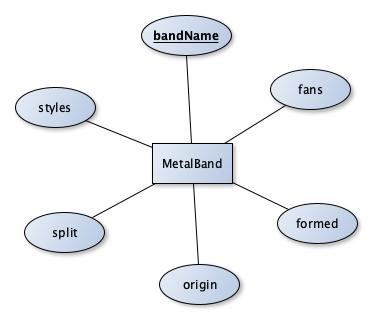
\includegraphics[width=0.4\textwidth]{g2-metal.jpg}}\qquad
    \subfloat[Terrorism\label{fig:terrorism}]{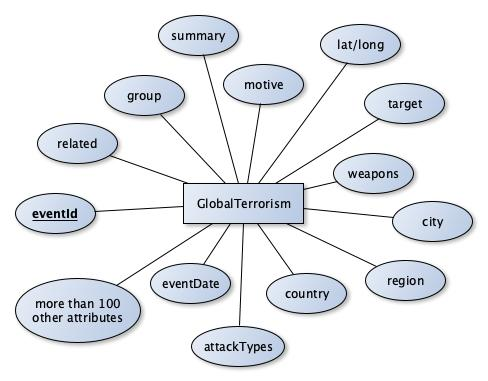
\includegraphics[width=0.45\textwidth]{g2-terror.jpg}}\qquad
    \subfloat[Country\label{fig:country}]{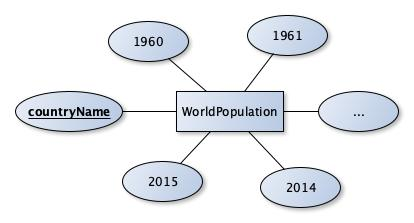
\includegraphics[width=0.35\textwidth]{g2-country.jpg}}\qquad
    \subfloat[Weather\label{fig:weather}]{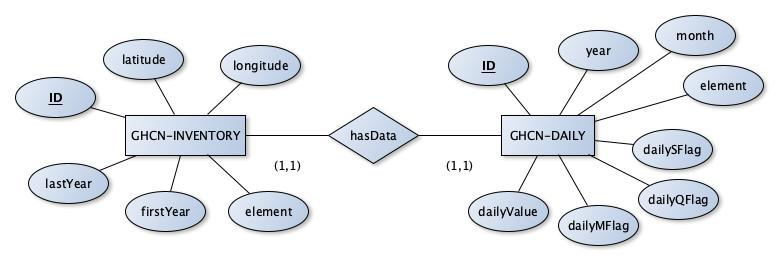
\includegraphics[width=0.55\textwidth]{g2-weather.jpg}}\qquad
    \caption{Entity-Relation diagrams of single sources}
\label{fig:example subfigure}
\end{figure}




\section{Integrated Schema}
A new Population Entity replaces the year attribute in Country. Some of the Terror data is outsourced to new Entities, as some attributes are listed data points. A new entity TerrorLocation is created to simplify relations with countries and weather data.

\subsection{ER}
\begin{figure}[hbt!]
	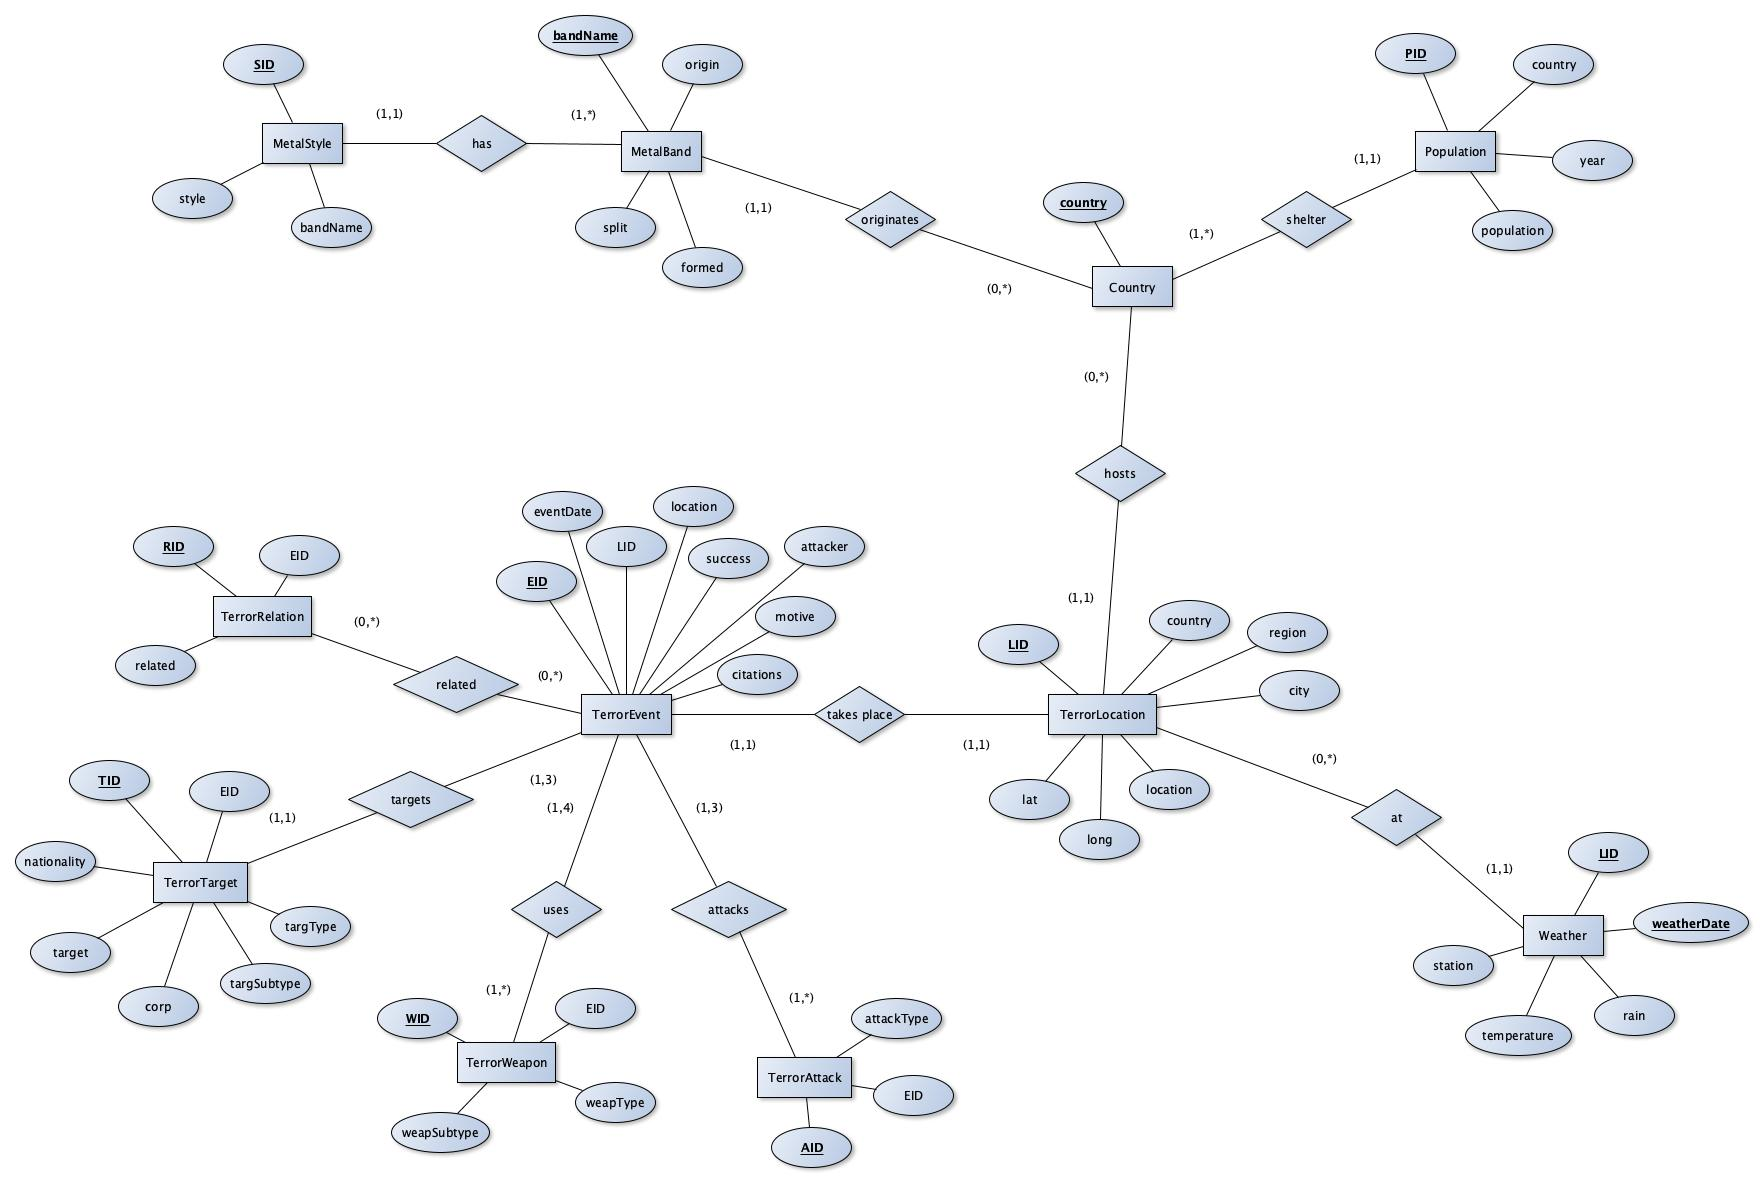
\includegraphics[width=\textwidth]{g2-integratedSchema.jpg}
	\caption{Entity-Relation diagram integrated schema}
\end{figure}
    
\subsection{Logical Schema}
\begin{itemize}
\item Country (\underline{countryName})
\item MetalBand (\underline{bandName}, formed, \uwave{origin}, split)
\item MetalStyle (\underline{SID}, \uwave{bandName}, style)
\item Population (\underline{PID}, \uwave{country}, year, population)
\item TerrorAttack (\underline{AID}, \uwave{EID}, attackTypeID, attackType)
\item TerrorEvent (\underline{EID}, eventDate, approxDate, extended, resolution, \uwave{LID}, summary, crit1, crit2, crit3, doubtterr, alternativeID, alternative, multiple, success, suicide, nkill, nkillus, nkillter, nwound, nwoundus, nwoundte, property, propextentID, propextent, propvalue, propcomment, addnotes, weapdetail, gname, gsubname, gname2, gsubname2, gname3, gsubname3, motive, guncertain1, guncertain2, guncertain3, individual, nperps, nperpcap, claimed, claimmodeID, claimmode, claim2, claimmode2ID, claimmode2, claim3, claimmode3ID, claimmode3, compclaim, ishostkid, nhostkid, nhostkidus, nhours, ndays, divert, country, ransom, ransomamt, ransomamtus, ransompaid, ransompaidus, ransomnote, hostkidoutcomeID, hostkidoutcome, nreleased, scite1, scite2, scite3, dbsource, INT\_LOG, INT\_IDEO, INT\_MISC, INT\_ANY)
\item TerrorLocation (\underline{LID}, countryID, \uwave{country}, regionID, region, provstate, city, latitude, longitude, specificity, vicinity, location)
\item TerrorRelation (\underline{RID}, \uwave{EID}, {related})
\item TerrorTarget (\underline{TID}, \uwave{EID}, targTypeID, targType, targSubtypeID, targSubtype, corp, target, nationalityID, nationality)
\item TerrorWeapon (\underline{WID}, \uwave{EID}, weapTypeID, weapType, weapSubtypeID, weapSubtype)
\item Weather (\underline{\uwave{LID}, weatherDate}, rain, temperature, station)
\end{itemize}

